\documentclass[12pt]{article}
\setlength{\oddsidemargin}{0in}
\setlength{\evensidemargin}{0in}
\setlength{\textwidth}{6.5in}
\setlength{\parindent}{0in}
\setlength{\parskip}{\baselineskip}

\usepackage[letterpaper, portrait, margin=1in]{geometry}
\usepackage[usenames, dvipsnames, rgb]{xcolor}
\usepackage{amsmath,amsfonts,amssymb,circuitikz,pdfpages,tikz,fancyvrb}
\usepackage{tikz-timing}

\usetikzlibrary{matrix,calc,circuits.logic.US, shapes.geometric}
\tikzstyle{branch}=[fill, shape=circle, minimum size=3pt, inner sep=0pt]
\tikzstyle{mux} = [ trapezium,   draw,
                    shape border rotate = 270, trapezium angle = 60,
                    inner ysep=0pt, outer sep=1pt, inner xsep=1pt,
                    text width = 1.5em, align = center,
                    node distance=3cm]


\newcommand{\overbar}[1]
    {\mkern1.5mu\overline{\mkern-1.5mu#1\mkern-1.5mu}\mkern1.5mu}

\begin{document}

\renewcommand{\arraystretch}{1.25}

\makeatletter
    \pgfdeclareshape{tff}{
      \savedanchor\northeast{%
        \pgfmathsetlength\pgf@x{\pgfshapeminwidth}%
        \pgfmathsetlength\pgf@y{\pgfshapeminheight}%
        \pgf@x=0.5\pgf@x
        \pgf@y=0.5\pgf@y
      }
      % This is redundant, but makes some things easier:
      \savedanchor\southwest{%
        \pgfmathsetlength\pgf@x{\pgfshapeminwidth}%
        \pgfmathsetlength\pgf@y{\pgfshapeminheight}%
        \pgf@x=-0.5\pgf@x
        \pgf@y=-0.5\pgf@y
      }
      \inheritsavedanchors[from=rectangle]
      \inheritanchorborder[from=rectangle]
      \anchor{center}{\pgfpointorigin}
      \anchor{north}{\northeast \pgf@x=0pt}
      \anchor{east}{\northeast \pgf@y=0pt}
      \anchor{south}{\southwest \pgf@x=0pt}
      \anchor{west}{\southwest \pgf@y=0pt}
      \anchor{north east}{\northeast}
      \anchor{north west}{\northeast \pgf@x=-\pgf@x}
      \anchor{south west}{\southwest}
      \anchor{south east}{\southwest \pgf@x=-\pgf@x}
      \anchor{T}{
        \pgf@process{\northeast}%
        \pgf@x=-1\pgf@x%
        \pgf@y=.5\pgf@y%
      }
      \anchor{CLK}{
        \pgf@process{\northeast}%
        \pgf@x=-1\pgf@x%
        \pgf@y=-.5\pgf@y%
      }
      \anchor{Q}{
        \pgf@process{\northeast}%
        \pgf@y=.5\pgf@y%
      }
      \anchor{Qn}{
        \pgf@process{\northeast}%
        \pgf@y=-.5\pgf@y%
      }

      \backgroundpath{
        % Rectangle box
        \pgfpathrectanglecorners{\southwest}{\northeast}
        % Angle (>) for clock input
        \pgf@anchor@tff@CLK
        \pgf@xa=\pgf@x \pgf@ya=\pgf@y
        \pgf@xb=\pgf@x \pgf@yb=\pgf@y
        \pgf@xc=\pgf@x \pgf@yc=\pgf@y
        \pgfmathsetlength\pgf@x{1.6ex} % size depends on font size
        \advance\pgf@ya by \pgf@x
        \advance\pgf@xb by \pgf@x
        \advance\pgf@yc by -\pgf@x
        \pgfpathmoveto{\pgfpoint{\pgf@xa}{\pgf@ya}}
        \pgfpathlineto{\pgfpoint{\pgf@xb}{\pgf@yb}}
        \pgfpathlineto{\pgfpoint{\pgf@xc}{\pgf@yc}}
        \pgfclosepath

        \begingroup

        \pgf@anchor@tff@T
        \pgftext[left,base,at={\pgfpoint{\pgf@x}{\pgf@y}},
          x=\pgfshapeinnerxsep]{\raisebox{-0.75ex}{T}}

        \pgf@anchor@tff@Q
        \pgftext[right,base,at={\pgfpoint{\pgf@x}{\pgf@y}},
          x=-\pgfshapeinnerxsep]{\raisebox{-.75ex}{Q}}

        \pgf@anchor@tff@Qn
        \pgftext[right,base,at={\pgfpoint{\pgf@x}{\pgf@y}},
          x=-\pgfshapeinnerxsep]{\raisebox{-.75ex}{$\overline{\mbox{Q}}$}}

        \endgroup
      }
    }
    % Key to add font macros to the current font
    \tikzset{add font/.code={\expandafter\def\expandafter\tikz@textfont
            \expandafter{\tikz@textfont#1}}}

    % Define default style for this node
    \tikzset{flip flop/port labels/.style={font=\sffamily\scriptsize}}
    \tikzset{every tff node/.style={draw,minimum width=1.5cm,
            minimum height=2.25cm,very thick,inner sep=1mm,outer sep=0pt,
            cap=round,add font=\sffamily}}
\makeatother

\makeatletter
    \pgfdeclareshape{dff}{
      \savedanchor\northeast{%
        \pgfmathsetlength\pgf@x{\pgfshapeminwidth}%
        \pgfmathsetlength\pgf@y{\pgfshapeminheight}%
        \pgf@x=0.5\pgf@x
        \pgf@y=0.5\pgf@y
      }
      % This is redundant, but makes some things easier:
      \savedanchor\southwest{%
        \pgfmathsetlength\pgf@x{\pgfshapeminwidth}%
        \pgfmathsetlength\pgf@y{\pgfshapeminheight}%
        \pgf@x=-0.5\pgf@x
        \pgf@y=-0.5\pgf@y
      }
      \inheritsavedanchors[from=rectangle]
      \inheritanchorborder[from=rectangle]
      \anchor{center}{\pgfpointorigin}
      \anchor{north}{\northeast \pgf@x=0pt}
      \anchor{east}{\northeast \pgf@y=0pt}
      \anchor{south}{\southwest \pgf@x=0pt}
      \anchor{west}{\southwest \pgf@y=0pt}
      \anchor{north east}{\northeast}
      \anchor{north west}{\northeast \pgf@x=-\pgf@x}
      \anchor{south west}{\southwest}
      \anchor{south east}{\southwest \pgf@x=-\pgf@x}
      \anchor{D}{
        \pgf@process{\northeast}%
        \pgf@x=-1\pgf@x%
        \pgf@y=.5\pgf@y%
      }
      \anchor{CLK}{
        \pgf@process{\northeast}%
        \pgf@x=-1\pgf@x%
        \pgf@y=-.5\pgf@y%
      }
      \anchor{Q}{
        \pgf@process{\northeast}%
        \pgf@y=.5\pgf@y%
      }
      \anchor{Qn}{
        \pgf@process{\northeast}%
        \pgf@y=-.5\pgf@y%
      }

      \backgroundpath{
        % Rectangle box
        \pgfpathrectanglecorners{\southwest}{\northeast}
        % Angle (>) for clock input
        \pgf@anchor@dff@CLK
        \pgf@xa=\pgf@x \pgf@ya=\pgf@y
        \pgf@xb=\pgf@x \pgf@yb=\pgf@y
        \pgf@xc=\pgf@x \pgf@yc=\pgf@y
        \pgfmathsetlength\pgf@x{1.6ex} % size depends on font size
        \advance\pgf@ya by \pgf@x
        \advance\pgf@xb by \pgf@x
        \advance\pgf@yc by -\pgf@x
        \pgfpathmoveto{\pgfpoint{\pgf@xa}{\pgf@ya}}
        \pgfpathlineto{\pgfpoint{\pgf@xb}{\pgf@yb}}
        \pgfpathlineto{\pgfpoint{\pgf@xc}{\pgf@yc}}
        \pgfclosepath

        \begingroup

        \pgf@anchor@dff@D
        \pgftext[left,base,at={\pgfpoint{\pgf@x}{\pgf@y}},
          x=\pgfshapeinnerxsep]{\raisebox{-0.75ex}{D}}

        \pgf@anchor@dff@Q
        \pgftext[right,base,at={\pgfpoint{\pgf@x}{\pgf@y}},
          x=-\pgfshapeinnerxsep]{\raisebox{-.75ex}{Q}}

        \pgf@anchor@dff@Qn
        \pgftext[right,base,at={\pgfpoint{\pgf@x}{\pgf@y}},
          x=-\pgfshapeinnerxsep]{\raisebox{-.75ex}{$\overline{\mbox{Q}}$}}

        \endgroup
      }
    }
    % Key to add font macros to the current font
    \tikzset{add font/.code={\expandafter\def\expandafter\tikz@textfont
            \expandafter{\tikz@textfont#1}}}

    % Define default style for this node
    \tikzset{flip flop/port labels/.style={font=\sffamily\scriptsize}}
    \tikzset{every dff node/.style={draw,minimum width=1.5cm,
            minimum height=2.25cm,inner sep=1mm,outer sep=0pt,
            cap=round,add font=\sffamily}}
\makeatother

\title{Digital Logic Homework 7}

ECEN 2350 Spring 2017 \hfill Homework 7\\
Samuel Cuthbertson

\hrulefill{}
\begin{enumerate}
  \item \textit{Book Problems: 5.7, 5.10, 5.16, 5.25}
  \begin{enumerate}
    \item[5.7:] \textit{Show how a JK flip-flop can be implemented with a T
                        flip-flop and other gates.}

      \vspace{3mm}
      Note that the characteristic equations for a T flip-flip and for a JK
        flip-flop are both shown below.
      \begin{center}
        \begin{minipage}{0.4\textwidth}
          \begin{center}
            \begin{tabular}{c | c}
                  T & $Q(t+1)$ \\
                  \hline
                  0 & $Q(t)$ \\
                  1 & $\overbar{Q(t)}$
            \end{tabular}
          \end{center}
        \end{minipage}
        \hfill
        \begin{minipage}{0.4\textwidth}
          \begin{center}
            \begin{tabular}{c c | c}
                  J & K & $Q(t+1)$ \\
                  \hline
                  0 & 0 & $Q(t)$ \\
                  0 & 1 & 0 \\
                  1 & 0 & 1 \\
                  1 & 1 & $\overbar{Q(t)}$
            \end{tabular}
        \end{center}
        \end{minipage}
      \end{center}
      \vspace{3mm}
      Therefor, for $J = K$ or $J \otimes K$, we can use J as T. For $J\neq K$,
        we need to set $T = J \oplus Q(t)$, as that will set $T=1$ when
        $Q(t) \neq J$ and will toggle $Q(t+1)$. This is implemented below.
      \begin{center}
        \begin{tikzpicture}[circuit logic US]
          %Inputs
          \node (J) at (0,6) {J};
          \node (K) at (0,5) {K};
          \node (CLK) at (0,4.185) {CLK};

          %Flip-flop
          \node[shape=tff, inner sep=2ex, draw] (TFF) at (10,4.75) {};

          %Gates
          \node[xor gate US, draw, logic gate inputs=nn] (JxorK) at (2,5.5){};
          \node[not gate US, draw,logic gate inputs=n](nJxorK)at(3.5,4.924){};
          \node[and gate US, draw, logic gate inputs=nn] (nJand) at (5,5) {};
          \node[xor gate US, draw, logic gate inputs=nn](JxorQ)at(5,6.075){};
          \node[and gate US, draw, logic gate inputs=nn](Qand)at(6.5,5.575){};
          \node[or gate US, draw, logic gate inputs=nn] (Tor) at (8,5.25) {};

          %Output
          \node (Q) at ($(TFF.Q) + (1.5,0)$) {$Q$};
          \node (nQ) at ($(TFF.Qn) + (1.5,0)$) {$\overbar{Q}$};

          %Connections
          \draw (CLK) -- ($(CLK) + (2.25,0)$) |- (TFF.CLK);

          \draw (J) -- ++(0:1) node[branch](jb){};
          \draw (jb) |- (JxorK.input 1);
          \draw (K) -- ++(0:1) |- (JxorK.input 2);

          \draw (jb) -- ++(0:3) node[branch](jb2){};
          \draw (jb2) |- (nJand.input 1);

          \draw (nJxorK.output) -- (nJand.input 2);
          \draw (JxorK) -- ++(0:0.75) node[branch](jb3){} |- (nJxorK.input);

          \draw (jb2) -- (JxorQ.input 2);
          \draw (TFF.Q) -- ++(0:.5) node[branch](q){} -- ++(90:1.25) --
            ++(180:7.25) -- ++(270:.41) -- (JxorQ.input 1);

          \draw (JxorQ.output) -| ++(0:.25) |- (Qand.input 1);
          \draw (jb3) -- (Qand.input 2);

          \draw (Qand.output) -- ++(0:.25) |- (Tor.input 1);
          \draw (nJand.output) -- ++(0:1.75) |- (Tor.input 2);

          \draw (Tor.output) -- ++(0:0.9) |- (TFF.T);

          \draw (TFF.Q) -- (Q);
          \draw (TFF.Qn) -- (nQ);

        \end{tikzpicture}
      \end{center}

    \item[5.10:] \textit{Write the behavioral Verilog code for a JK flip-flop.}

      \begin{Verbatim}
module jk_flip_flop(J, K, CLK, Q, nQ)
  input reg J, K, CLK;
  output reg Q, nQ;

  always@(posedge CLK)
  begin
    case({J, K})
      {1'b0, 1'b1}: Q <= 1'b0;
      {1'b1, 1'b0}: Q <= 1'b1;
      {1'b1, 1'b1}: Q <= ~Q;
    endcase
    nQ = ~Q
  end
endmodule
      \end{Verbatim}

    \item[5.16:] \textit{Design a three bit up/down counter using D flip-flops,
                        using a control signal of $\overbar{UP}/DOWN$.}

      For an up counter, we can use the equations $D_0 = Q_0 \oplus 1$,
        $D_1 = Q_1 \oplus Q_0$, $D_2 = Q_2 \oplus Q_1 Q_0$. For a down counter,
        the equations are similar: $D_0 = Q_0 \oplus 1$,
        $D_1 =\overbar{Q_0} \oplus Q_1 $, $D_2 = \overbar{Q_1} \oplus Q_1 Q_2$.
        As the only diffrence between these is whether to use $Q_{n-1}$ or
        $\overbar{Q_{n-1}}$ in the \texttt{xor} with the previous \texttt{and},
        we can use a \texttt{mux} at each stage with our control signal as a
        select.

      \begin{center}
        \begin{tikzpicture}[scale=.75, transform shape]
          %Inputs
          \node (CLK) at (-3, 1) {CLK};
          \node (CTRL) at (-1.75, 5.5) {$\overbar{UP}/DOWN$};

          %Q0
          \node[shape=dff, draw] (D0) at (0,3) {};
          \node[mux, draw] (M0) at (2.25,3.25) {0\\1};
          \node[xor gate US, draw, logic gate inputs=nn] (X0) at (4,3.34) {};
          \node (Q0o) at (1.32,7) {$Q_0$};

          %Q0 connections
          \draw (CTRL) -- ++(0:4) node[branch] (Q0CLB) {} -- (M0);
          \draw (D0.Q) -- ++(0:.57) node [branch] (Q0) {} -- ++(0:.57);
          \draw (D0.Qn) -- ++(0:.6) node [branch] (nQ0) {} |- (M0.south west);
          \draw (nQ0) -- ++(0,-1) node[branch] (nQ02){} -- ++(-2.5,0) |- (D0.D);
          \draw (CLK) -- ++(1.5,0) node [branch] (Q0CLK) {} |- (D0.CLK);
          \draw (M0) -- (X0.input 2);
          \draw (Q0) -- ++(0,1) node[branch] (Q02) {} -- (Q0o);

          %Q1
          \node[shape=dff, draw] (D1) at (6,3) {};
          \node[and gate US, draw, logic gate inputs=nn] (A11) at (8,3.64) {};
          \node[and gate US, draw, logic gate inputs=nn] (A12) at (8,2.35) {};
          \node[mux, draw] (M1) at (9.5,3.25) {0\\1};
          \node[xor gate US, draw, logic gate inputs=nn] (X1) at (11,3.34) {};
          \node (Q1o) at (7.05,7) {$Q_1$};

          %Q1 connections
          \draw (Q0CLB) -- ++(0:7.25) node[branch] (Q1CLB) {} -- (M1);
          \draw (X0.output) -- ++(.35,0) |- (D1.D);
          \draw (D1.Q) -- ++(0:.3) node[branch] (Q1) {} -- (A11.input 2);
          \draw (D1.Qn) -- (A12.input 1);
          \draw (A11.output) -- ++(0:.78);
          \draw (A12.output) -- ++(0:.4) -- ++(0,.5) -- ++(.4,0);
          \draw (Q0CLK) -- ++(6,0) node[branch] (Q1CLK) {} |- (D1.CLK);
          \draw (M1) -- (X1.input 2);
          \draw (nQ02) -- ++(0:6) |- (A12.input 2);
          \draw (Q02) -- ++(0:6) |- (A11.input 1);
          \draw (Q1) -- (Q1o);

          %Q2
          \node[shape=dff, draw] (D2) at (13,3) {};
          \node (Q2o) at (14.25,7) {$Q_2$};

          %Q2 connections
          \draw (X1.output) -- ++(.35,0) |- (D2.D);
          \draw (Q1CLK) -- ++(7,0) |- (D2.CLK);
          \draw (D2.Q) -- ++(.5,0) -- ++(0,1) node[branch] (Q2) {} -- (Q2o);
          \draw (Q2) -- ++(-4,0) |- (X1.input 1);

        \end{tikzpicture}
      \end{center}

    \item[5.25:] \textit{Using the circuit shown in the book, complete the
                         below timing diagram.}

      Placeholder answer

  \end{enumerate}

  \newpage
  \item \textit{Draw a 4-bit Universal shift register that can parallel load,
                shift left, shift right, and synchronously clear. Provide a
                characteristic table for the control operations.}

    Placeholder answer

  \newpage
  \item \textit{Implement a 3-bit up-counter using only one D flip-flop, one
                T flip-flop, one JK flip-flop and one AND gate. Assume all
                flip-flops are positive edge triggered. Show your circuit and
                a timing diagram.}

    You don't have a power source or a clock, so all of this is moot, but
      if you could find both of those then you could implement an up counter
      as shown below.

    As the first bit $Q_0$ changes with every posedge of clock, we can simply
      attach $\overbar{Q_0}$ to the input of the D and use that output for
      $Q_0$.

    Similarly, as $Q_1$ toggles between 1 and 0 every time
      $\overbar{Q_0}$ changes from 0 to 1 (posedge) we can attach 1 as the input
      to the T flip-flop and $\overbar{Q_0}$ to the clock, and then use the
      output from the T flip-flop as $Q_1$.

    Finally, as $Q_2$ toggles everytime that $\overbar{Q_0}\overbar{Q_1}$ goes
      0 to 1 (posedge), we can attach the output from that {\tt and} gate to
      both J and K, making the JK flip-flop behave like a T flip-flop. Then, we
      can use the output from the JK flip-flop as $Q_2$.

    All this put together is shown below:

    \begin{center}
      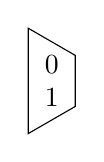
\begin{tikzpicture}
          \node[mux] (m) at (0,0) {0\\1};
      \end{tikzpicture}
    \end{center}

  \newpage
  \item \textit{Write the behavioural Verilog for 5.16, calling the module
                \texttt{up\_down\_counter}.}

    \begin{Verbatim}
module up_down_counter(clk, ctrl, value);
  input clk;
  input ctrl;
  output reg [2:0] value;

  always@(posedge clk)
  begin
    case(ctrl)
      1'b0: value <= value - 1;
      1'b1: value <= value + 1;
    endcase
  end
endmodule
    \end{Verbatim}
\end{enumerate}
\end{document}
